\documentclass[draftcopy]{srpaper}

\usepackage[toc,page]{appendix}
\usepackage{hyperref}
\usepackage[outputdir=latexmk]{minted}
\usepackage{pdfpages}
\usepackage{url}

\definecolor{bg}{rgb}{0.95,0.95,0.95}
\setminted{bgcolor=bg}

\title{Rust vs. D:\ Exploring the Possible Successors of C++}
\author{Andy Russell}
\date{\today}
\advisor{Professor Kim Bruce}

\abstract{The programming languages D and Rust aim to simplify the complex and
error-prone features of C++ while maintaining a similar level of performance.
This paper examines whether the languages succeed in their goal of easing the
development of safe code, specifically focusing on each language's compile-time
features and memory management techniques. C++, D, and Rust are evaluated on
both subjective and empirical criteria. In order to evaluate the success of
each language's design goals, I will implement a number of small programs that
encompass common tasks in systems programming, each in C++, D, and Rust. I will
then recruit volunteers with prior experience with C++ to attempt to implement
each program in D or Rust. Each volunteer will document his or her development
process in detail, particularly noting any errors or bugs that might be
encountered. Each error programmers will be tallied and categorized to analyze
whether a particular language makes it easier to avoid certain errors. I will
then evaluate each language on expressiveness and ease of development to
determine whether the language's design goals have been met.}

\begin{document}
\frontmatter

\listoflistings{}

\chapter{Introduction}

Systems programming is an extremely important part of computing today. The raw
speed and low-level access to hardware provided by languages of this nature are
necessary for embedded systems, networking, and gaming, and any number of other
applications. However, such power comes with inherent
danger\footnote{Throughout this paper, when I refer to a concept or feature as
``dangerous,'' I mean that it is error-prone or difficult to reason about,
especially if the errors that may arise from its use are resistant to
debugging.}.

Mistakes in managing memory can lead to run-time crashes or security
vulnerabilities such as buffer overflow or format string
attacks~\cite{Shahriar:2012:MPS:2187671.2187673}. While there are many tools
designed to allow programmers to catch such errors, the ideal solution would be
to eliminate the burden of manual memory management. Other languages such as
Java and C\#, inspired by this goal, have removed that need. However, due to
their dependence on a virtual machine, they have sacrificed performance and the
ability to interface directly with
hardware~\cite{Alexandrescu:2010:DPL:1875434}. The languages examined in this
paper, D and Rust, do not use a virtual machine or run-time. The languages aim
to match the low-level speed and power of C++ while attempting to make code
easier to write both from an expressiveness and correctness standpoint.

\chapter{Background}

In order to adequately discuss the design decisions that the implementors of
Rust and D have made, it is important to decide a context from which we can
compare them. Since both languages aim to occupy the same space as C++, I have
decided to compare the languages using C++ as a reference point.

\section{History}

Though C++, D, and Rust are all related, each language developed within quite
different historical contexts.

C++ was developed in the early '80s by Bjarne Stroustrup. Stroustrup wished to
bring high-level features such as classes, strong typing, and default arguments
to C. It attempts to provide the programmer with a one-to-one mapping of
built-in types to the hardware, while also offering flexible abstractions to
allow user-defined types to take advantage of the same facilities available to
the built-ins. Stroustrup himself outlined the design philosophy of C++ in two
points:

\begin{itemize}
\item \textit{Leave no room for a lower-level language below C++}
\item \textit{What you don't use you don't pay for}. This is also known as the
``zero-overhead principle''.
\end{itemize}

These principles serve to keep C++ close to its roots in C while maintaining
the abstractions that make it a high-level language~\cite{stroustrup2013the}.
C++ remains one of the most popular languages in the world.

D was created in 2001 by Walter Bright, and later developed by Digital Mars.
From the name, it is easy to see that D has drawn much inspiration from C++, as
C++ did from C. However, D has made a number of backwards-incompatible changes
from C++ in the process of achieving its design goals. The D website cites a
number of reasons why D is necessary. Most relevant to this paper are its
assertions about the inherent complexity in C++ due to the sheer number of
features present in the language, the burden of explicit memory management,
memory, the difficulty in tracking down pointer bugs, and the hindrance of
backwards compatibility with C~\cite{Doverview}. D, while less popular than
C++, maintains a healthy online presence and is often advocated by C++ gurus
such as Andrei Alexandrescu.

Rust is a quite new programming language developed primarily by Mozilla
starting in 2012. Rust aims to give programmers enough power to access the
computer's hardware while providing ``strong guarantees about isolation,
concurrency, and memory safety''~\cite{Matsakis:2014:RL:2663171.2663188}.
Syntactically, Rust is a more radical departure from C++ than D. However, it
has similar design goals. Despite not having a stable release, Rust generates
a considerable amount of discussion and written code.

\section{Macros, Preprocessing, and Conditional Compilation}

The C++ macro preprocessor is an integral part of the language. Perhaps the
most common use of the feature is to \texttt{include} one file (the ``header'')
within another. By defining the interface in the header, the implementation is
kept inside a single source file, and any number of other source files may use
the interface's implementation. While the macro preprocessor is a necessary
part of the language, it is inherently dangerous. The preprocessor works by
modifying the actual text of the program, which can lead to syntax errors or
subtle bugs that are difficult to solve. Another use of the preprocessor is
for conditional compilation, where different code should be compiled depending
on various conditions such as the underlying architecture or character-encoding
support. Stroustrup advises that the C++ preprocessor should only be used for
these cases~\cite{stroustrup2013the}.

D also has an answer for the C++ preprocessor. The language contains a number
of features that obviate its need. For example, inclusion is handled by
modules, which handle imports of symbols from other files. This also removes
the need for include guards, because each symbol is only guaranteed to be
imported once. Conditional compilation is achieved through the
\texttt{version} keyword. D also contains an aggressive inliner, which removes
the need to implement small functions as macros~\cite{pretod}.

In lieu of the preprocessor, Rust has an extremely powerful macro system.
Rust macros operate on the abstract syntax tree of the program, rather than on
the text. This allows macros to be type-safe and extend the language itself.
In Rust, \texttt{println} is a macro that performs type-checking on its
arguments to ensure that the format string contains the proper number of
format placeholders for the arguments. In other languages, it might be
possible to check this with a special code path in the compiler, but in Rust
the language itself does the checking.


\section{Memory Management}

C++'s memory management is similar in some respects to its ancestor, C. Instead
of requesting and returning blocks of memory from the free store by use of
\texttt{malloc()} and \texttt{free()}, a C++ programmer uses \texttt{new} and
\texttt{delete}\footnote{C++ has separate operators for array allocation:
    \texttt{new[]} and \texttt{delete[]}.}. The language inherits the
requirement that the programmer must remember to \texttt{delete} all memory
acquired by \texttt{new} to avoid memory leaks, and that the programmer should
refrain from using deallocated or unallocated memory to prevent invoking
undefined behavior~\cite{stroustrup2013the}. Undefined behavior is
characterized by the \textit{lack} of a definition of what an implementation of
C++ should do in a given situation~\cite{iso/iec}. In other words, if a program
incurs undefined behavior, then an implementation is in no way required to act
in any particular way. The program may not compile, may crash at run-time, or
act in any number of ways. Clearly it is impossible to reason about the
correctness of a program that causes undefined behavior, so C++ programmers
must avoid it at all costs.

C++ programmers are well-aware of the problems that arise from using
\texttt{new} and \texttt{delete} improperly. In fact, Stroustrup warns that
``naked \texttt{new}'' (using \texttt{new} to allocate an object directly)
ought to be avoided. Instead, he advises programmers to use stack-based
allocation when possible, and in other cases use manager objects such as
\texttt{unique\_ptr} and \texttt{shared\_ptr}\footnote{These containers were
    introduced in C++11.}. This idiom is known as ``Resource Acquisition Is
Initialization'', or RAII~\cite{stroustrup2013the}. These containers help
abstract memory management away from the programmer by ensuring \texttt{delete}
is called when the pointer goes out of scope.

D handles memory management through its garbage collector. Classes are
automatically allocated on the heap, and all other data is created on the
stack. The garbage collector frees any memory that has gone out of scope
(though not necessarily immediately after). This removes the need for the
programmer to explicitly allocate and deallocate memory. If the programmer
wishes to obtain RAII behavior, D provides syntax to execute code after
variables go out of scope through destructors and scope guards~\cite{cppford}.

One of the interesting features of Rust is its guarantees about heap access.
Listing~\ref{lst:rustheapalloc} shows how one might allocate an int on the
heap in Rust.

\begin{listing}[H]
\begin{minted}{rust}
let x = Box::new(5i);
\end{minted}
\caption{Rust heap allocation.}
\label{lst:rustheapalloc}
\end{listing}

This code acts similarly to a \texttt{unique\_ptr} would in C++. It guarantees
that you cannot forget to free the memory, and that the memory is not used
after the free. Rust's semantics are more powerful than this, however. Rust
guarantees that ``no other writable pointers alias to this heap memory'',
meaning that it is impossible for multiple objects to write to this memory
(unless the programmer were to use an \texttt{Rc} pointer, which allows
multiple readers)~\cite{RustPointerGuide}.

\chapter{Evaluation Strategy}

\section{Criteria}

One of the most challenging aspects of evaluating languages is deciding the
criteria on which they are evaluated. In order to obtain as comprehensive an
evaluation of Rust and D as possible, I wish to include both qualitative and
quantitative criteria.

AlGhamdi and Urban provide an excellent list of qualitative methodologies on
which I have based the my own
methodology~\cite{AlGhamdi:1993:CAP:162754.162876}. Their paper summarizes
twelve methodologies, and the factors that may be used to achieve an apt
comparison. The following list summarizes the methodologies expounded in their
paper that I will employ in my project.

\begin{enumerate}
\item Comparison of Philosophy and History

Since both Rust and D occupy a similar domain, the main factor that I will use
to distinguish the two is the ``intention of [the] designers''. While these
languages were created nearly a decade apart, differ in their corporate
affiliations, and have varying development team size, I do not find these
factors relevant for my study. When evaluating the languages on their own, I
believe that the only factor that remains inherent in the language is its
philosophy.

\item The Degree of Permissiveness of the Language

This methodology includes criteria such as the ability of the programmer to
circumvent type-checking, operator overloading, and run-time checking. I am
particularly interested in the memory safety of Rust and D compared to C++.
While these languages will \textit{allow} a programmer to circumvent the type
system or perform unsafe memory accesses, such practices are discouraged. So,
I am interested in the effectiveness of each language in avoiding the
requirement of such practices.

\item Language Contributions to Program Readability

It is often said that code is read far more than it is written. In large
systems that depend on reliability, this is surely true. It follows that if
code is easier to read, it is easier to locate defects or bugs.

\item Language Contributions to Program Reliability

This is perhaps the most important methodology to my project. I am particularly
interested in examining how Rust and D attempt to avoid the common pitfalls
that plague C++ development. These include but are not limited to uninitialized
variables, null pointers, and memory leaks.

\item Data Structuring Facilities

This methodology is also quite important to my study. Rust and D are both
strongly typed, and each language provides a number of ways to inform the
compiler of programmer intent for the usage of various data types. Exploring
the numerous primitive data types is integral to understanding the power of
each language.

\item Control Facilities

I am particularly interested in procedural-level control facilities. This
includes parameter-passing methods, concurrency, and generics/templates.

\item Language Contributions to Program Cost

This methodology explores the various costs involved with writing in a language
under consideration. This involves the cost of learning the language, the cost
of writing a program in the language, and even the cost of compiling a program.
The cost of executing and maintaining a program is irrelevant for this paper,
but I imagine the maintainence cost is somewhat encompassed by the criteria for
evaluating the languages' readability. While this methodology is particularly
important for new programmers, and becomes less apparent with experience, it is
nonetheless important to consider.

\end{enumerate}

In contrast to the methodologies listed above, I found a number of
methodologies irrelevant. For example, D and Rust appear almost identical in
terms of modularity (``Language Contributions to Program Modularity''),
portability (``Portability of a Language''), I/O facilities (``Input/Output''),
and support for inline assembly and foreign functions (``Escape from a
Language''). These methodologies either contribute little to my goal of
studying the memory safety of Rust and D, or the features provided by each
language are so similar that there is little comparison to be made between the
two.

\section{Experimental Design}

While I believe that the aforementioned methodologies comprise a satisfactory
qualitative evaluation strategy for Rust and D, I do not believe that a full
comparison can be achieved with these methodologies alone. Furthermore, much of
the criteria is rather subjective. For my project, I have strived to develop a
method which can be used to compare various language features while avoiding
subjectivity or bias.

Originally, I planned to come up with a number of programs that embodied the
core of systems programming, and then develop these programs in C++, D, and
Rust. Then, using my own experiences, I would attempt to evaluate the
effectiveness of each language for developing these programs. However, this
approach is flawed in a number of ways. For example, perhaps I had attempted to
implement a program with logic that requires a large amount of conditionals in
Rust. I would likely have encountered a number of bugs with my initial
implementation, but then eventually come up with a satisfactory result. Then,
upon moving onto D, I would have avoided most of the errors that I encountered
while working on the Rust implementation. My development process in D would
likely have felt more natural, and the code would probably look eerily like
Rust. To mitigate this problem, I instead recruited a number of volunteers to
learn each language individually, and implement a series of programs meant to
demonstrate various features that are important to systems languages.

I advertised my study both on the Computer Science Facebook group and through
Computer Science colloquium. Once volunteers indicated their interest, I sent
them a document\footnote{The document may be found online at
\url{https://github.com/euclio/senior-project/blob/master/resources/project_agreement.md}}
detailing my expectations for the project. The volunteers then sent me
information including their name, major, experience with programming, and a
confirmation that they read the document in its entirety.

Each volunteer was then assigned either Rust or D as a language. I tried to
satisfy the volunteer's preference for learning the language, though I first
ensured that the experience level between each language would be comparable.
Over the next month, each volunteer was expected to attempt to implement one
of five programs. The volunteers were not expected to spend more than 2 hours
on each program, but most volunteers worked on each program to completion.

The programs implemented by the volunteers were designed to cover an
assortment of language features as well as highlighting common bugs. The
programs were as follows:

\begin{enumerate}

\item Sentence Splitter

Volunteers were asked to implement a single string into sentences using a set
of heuristics. The difficulty of this program stems from the fact that
while sentences are delimited by periods, question marks, and exclamation
points, they may also include websites, titles, and abbreviations, all of
which are \textit{not} boundaries.

This program was meant to introduce the programmers to string manipulation
techniques and required a large amount of logical branching.

\item Integer Linked List

The next program was to implement a simple linked list data structure that
operates on integers. A number of operations were required to be supported,
including insertion, deletion, retrieval, and methods to query the size, head
and tail of the list.

This program introduced the volunteers to object-orientation, pointer
manipulation, and memory allocation.

\item Generic Array List

The next program involved creating an array list that supported generic
elements. The array list was required to support the same operations as the
integer linked list, and covered the same features of the languages.

\item Parallel Mergesort

Volunteers were then asked to implement the parallel mergesort algorithm. This
algorithm is relatively simple to understand, and easily parallelizable.

This program introduced the programmers to recursion and concurrency.

\item Brainfuck [sic] Interpreter

Lastly, the programmers were asked to implement a Brainfuck interpreter.
Brainfuck is an esoteric programming language, known for being fiendishly
unreadable. However, the language's semantics are quite easy to understand. In
short, there are eight meaningful characters in the language, all of which
either manipulate the ``data pointer'' in some way (by incrementing,
decrementing, etc.), or perform I/O on the byte pointed at by the pointer.

This program served as a kind of ``capstone'' for the study. It is larger than
the other programs, and involves file I/O and involved pointer manipulation.

\end{enumerate}

Each volunteer was also required to document their development process. While
developing each program, the volunteer would note every error encountered,
categorize it as a syntax error, logic error, or resource error, and whether
the error was caught at compile-time or run-time.

\chapter{Results}

\chapter{Conclusion}

\nocite{*}
\bibliography{senior-project}

\begin{appendices}
\chapter{Volunteer Resources}
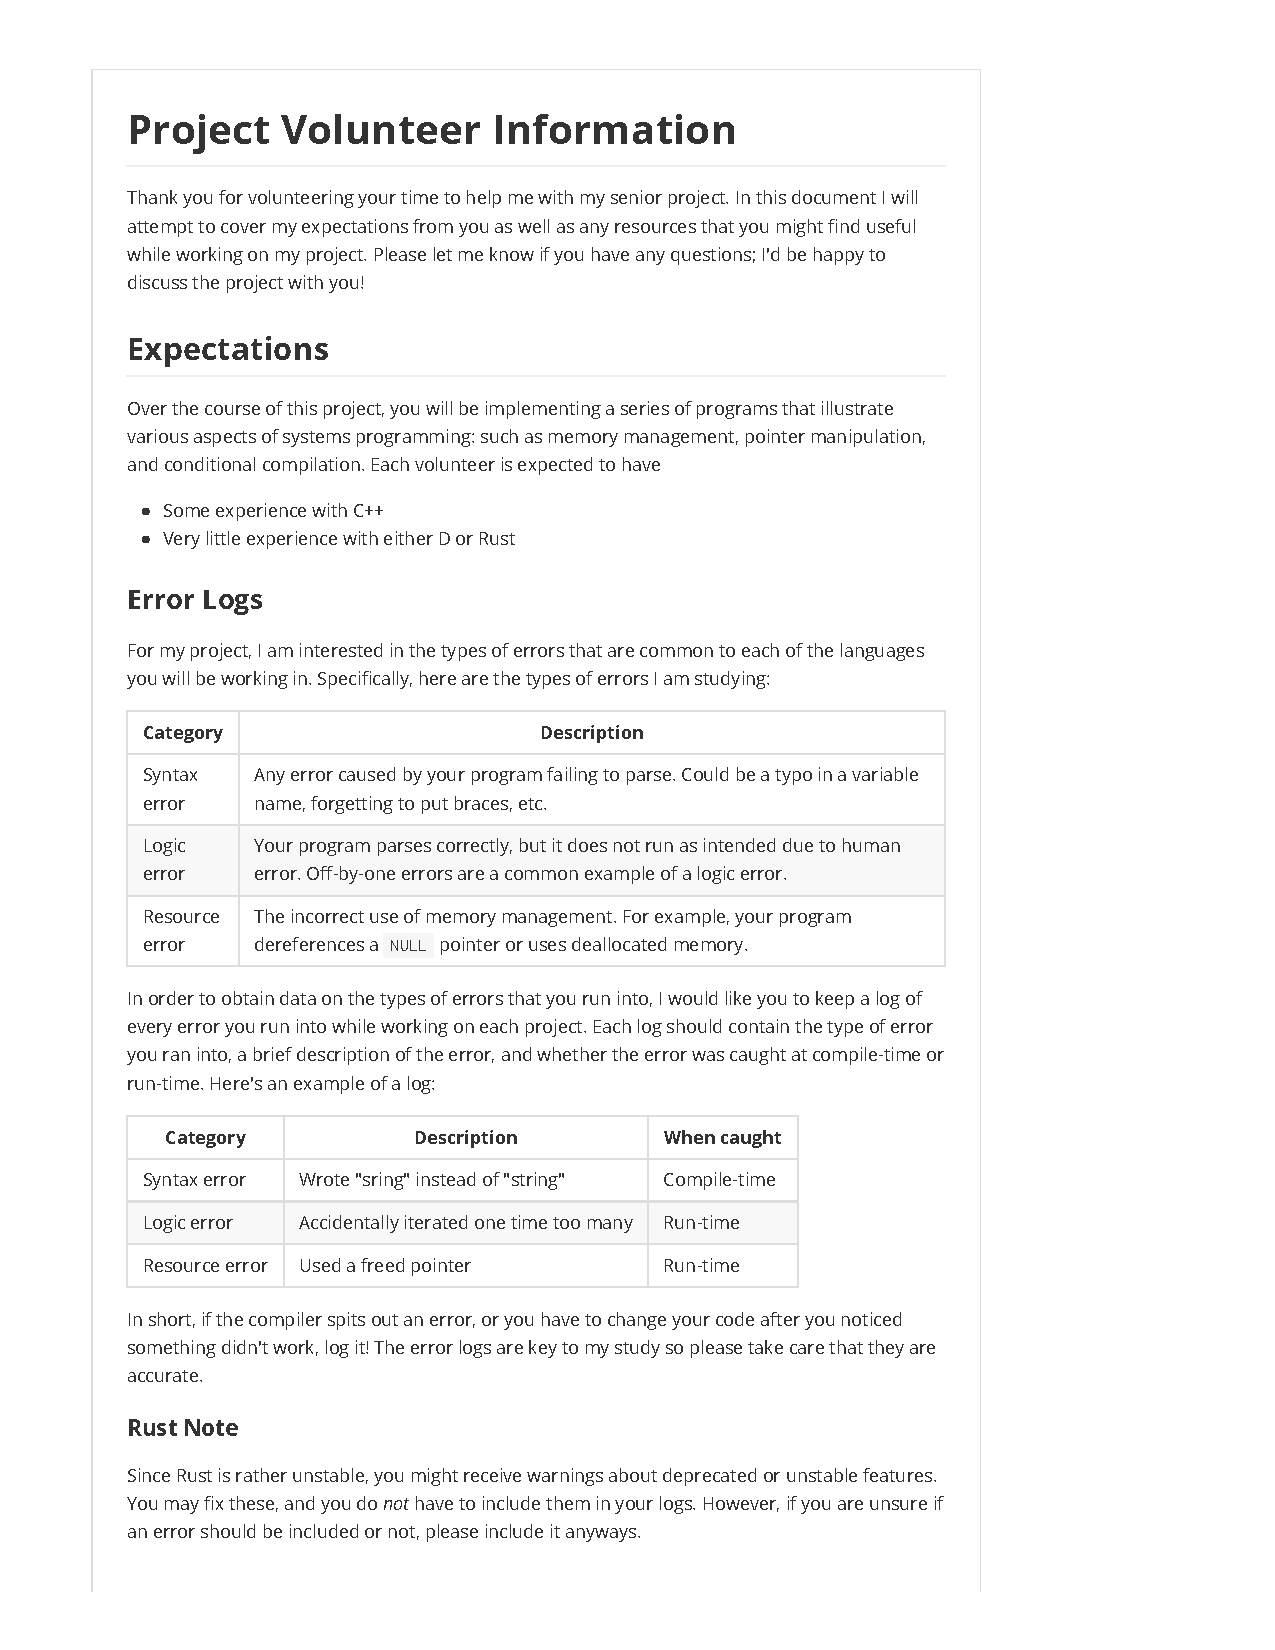
\includepdf[pages={-}]{../resources/project_agreement.pdf}
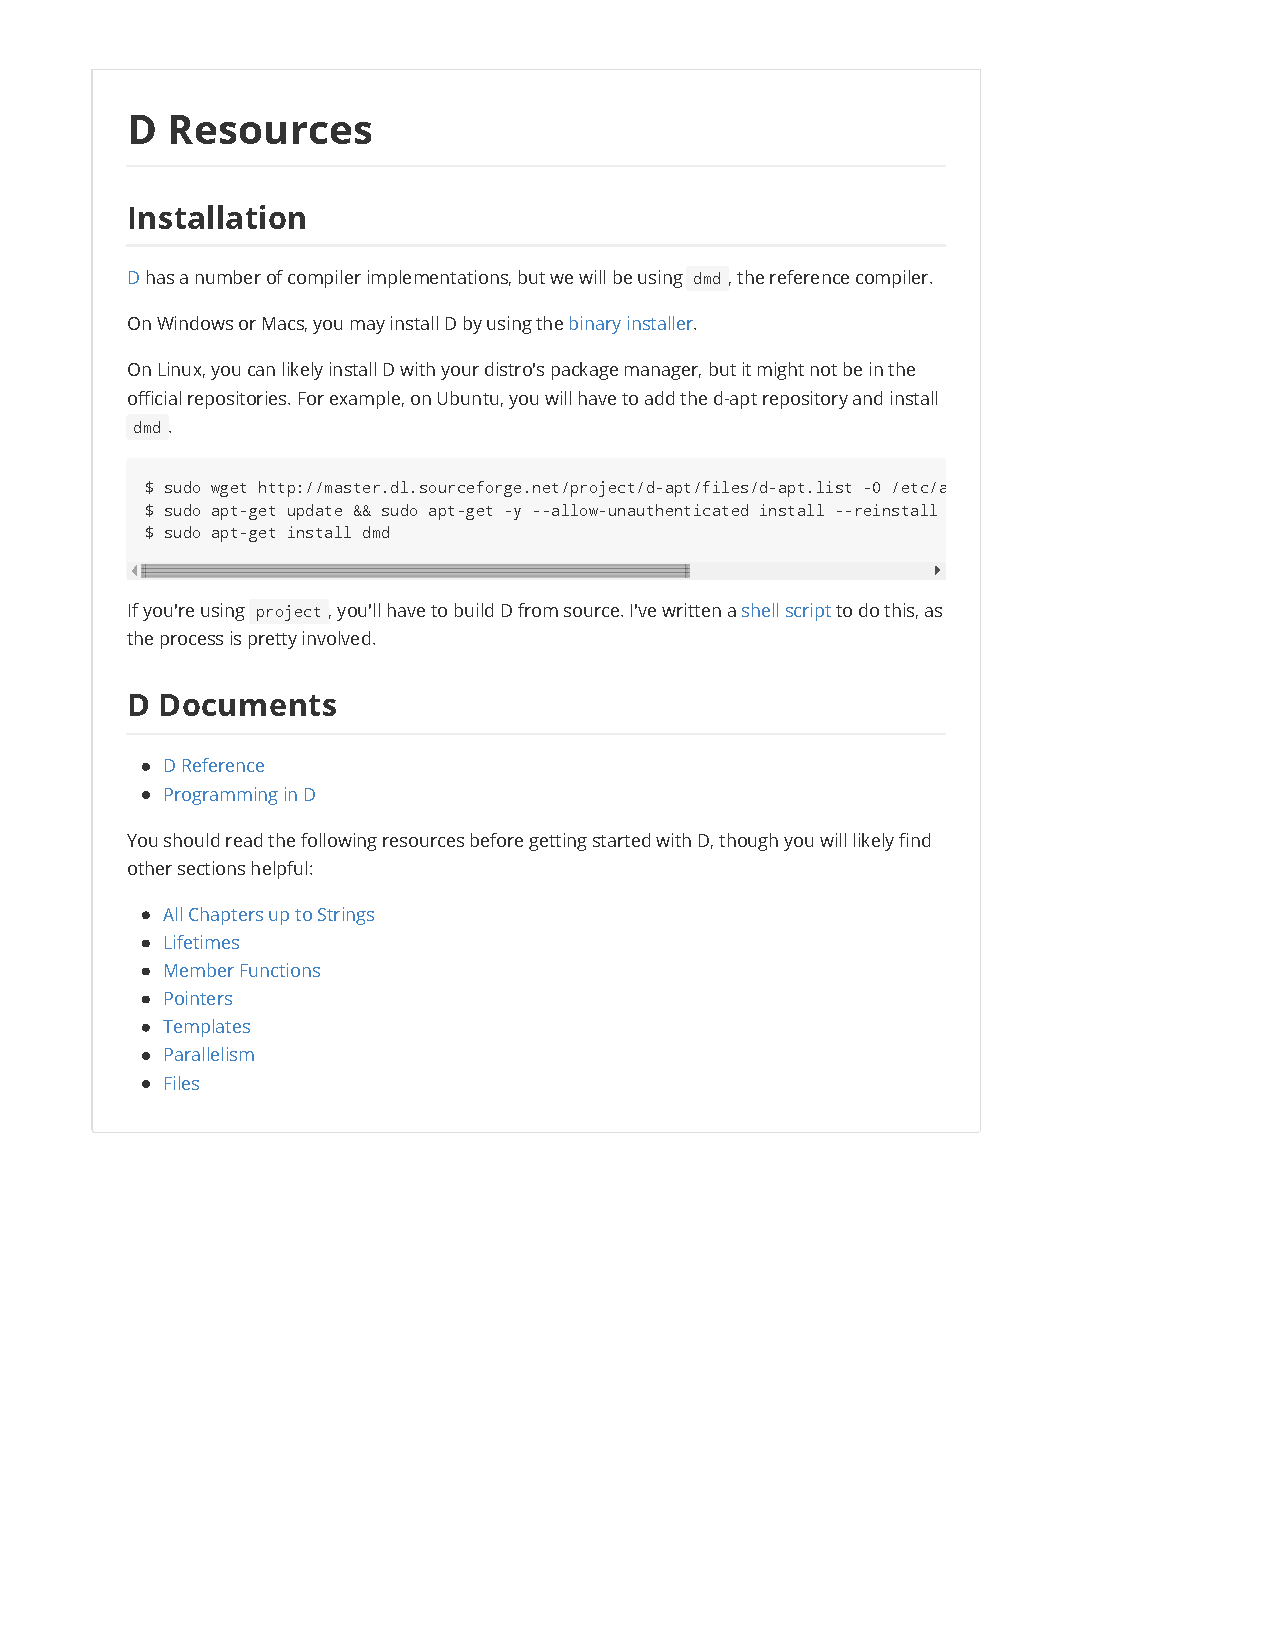
\includepdf[pages={-}]{../resources/d_resources.pdf}
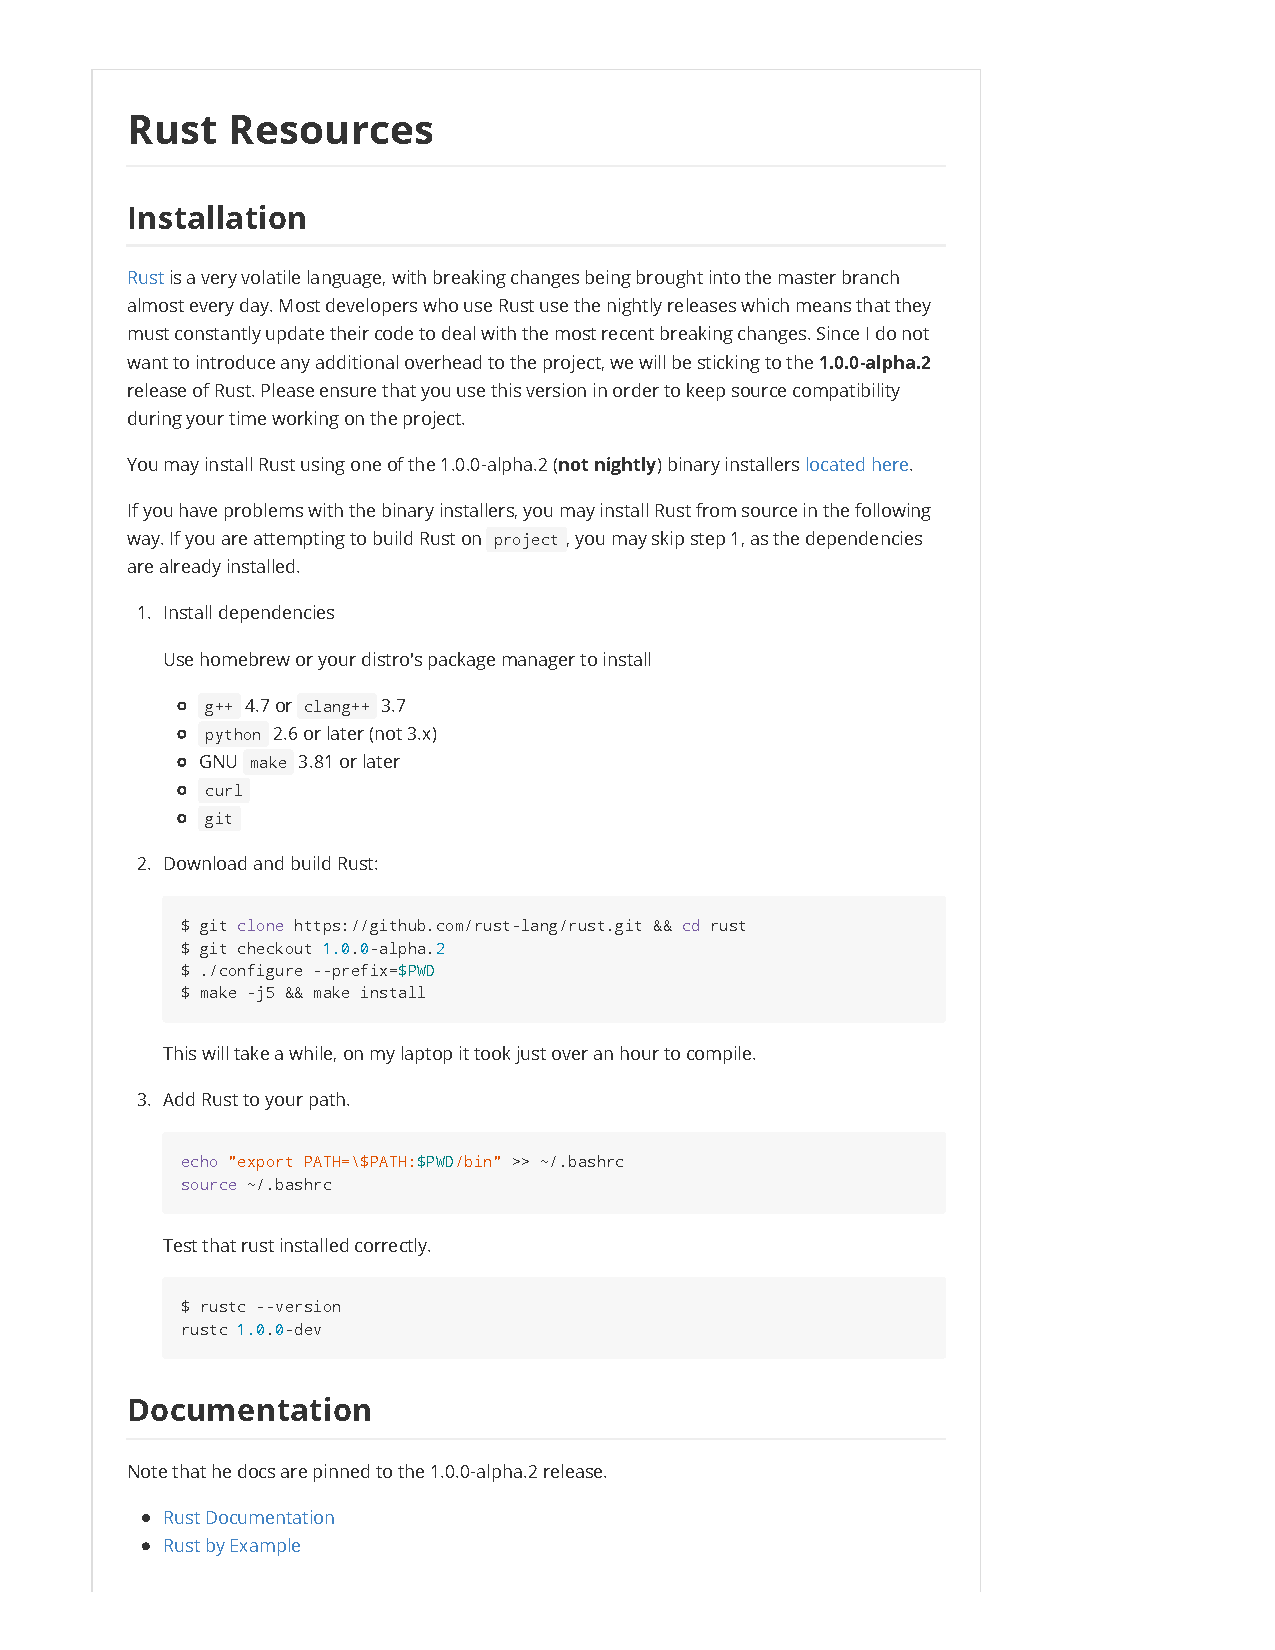
\includepdf[pages={-}]{../resources/rust_resources.pdf}
\end{appendices}

\end{document}
